\section{Case Study\label{sec:casestudy}: visual exploration of topic modeling in RCloud}

LDAVis helps non-experts to explore collections of
short text documents, using topic modeling and
visualization. Topic modeling~\cite{Blei:2003:LDA},
although powerful, often requires human guidance
and interpretation~\cite{Sievert:2014:LAM}.

\begin{figure*}
  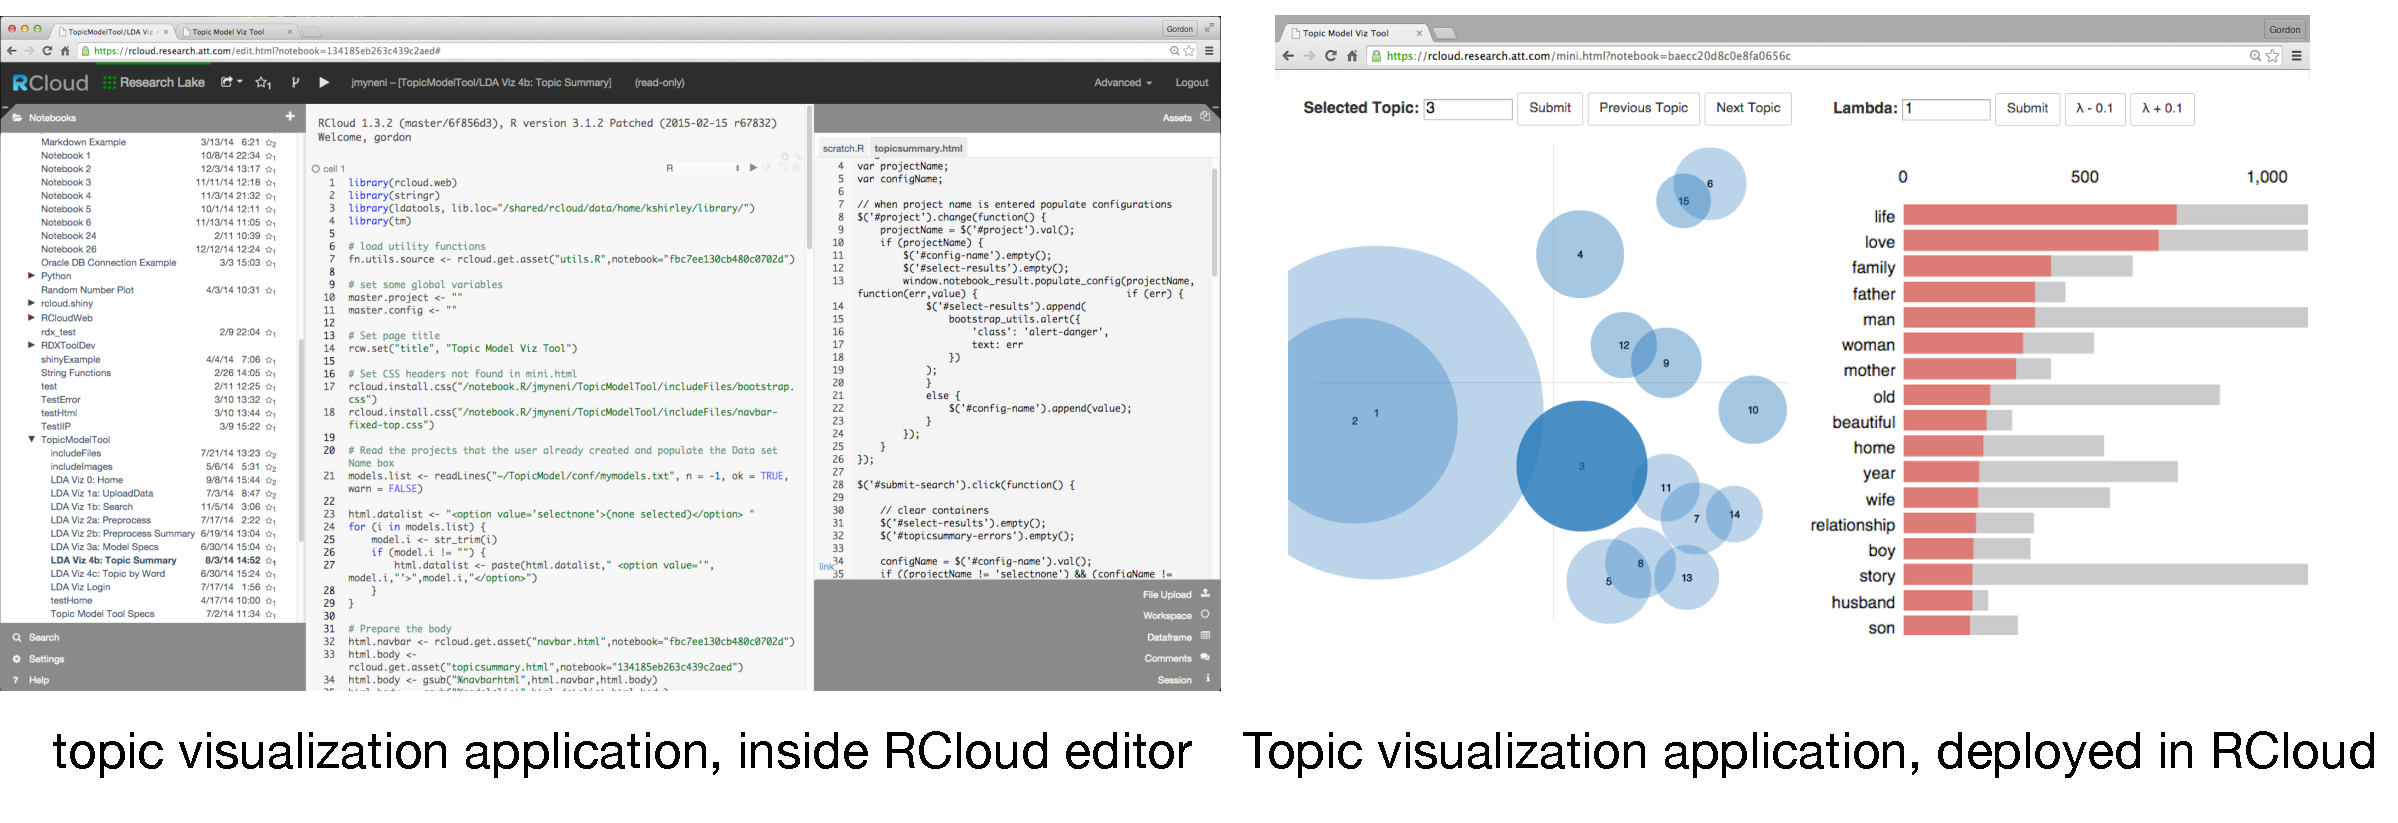
\includegraphics[width=\linewidth]{fig/casestudytext/casestudytext.pdf}
  \caption{\label{fig:textvis}An example application developed and deployed in RCloud.}
\end{figure*}

LDAVis was developed by two technical staff members at
AT\&T Labs, originally in RStudio Shiny~\cite{RStudio:2013:SWA},
a framework for developing web applications in R.
While Shiny offers outstanding ease of development,
discoverability and deployment are also very important aspects
in an application's lifecycle (see Section~\ref{sec:interviews}).
RCloud's assumption that \emph{all developed notebooks are automatically
deployed} simplifies this for LDAVis.

LDAVis combines text analysis, dimensionality reduction and
interactive visualization. Text analysis is performed by
combining a standard R library to fit LDA models using
Gibbs sampling~\cite{} with custom R code written by the
developers. The analysis module is a single R function
exposed to the web application via the Javascript-R RPC
mechanism described in Section~\ref{sec:system};
thus analysis is performed remotely on an RCloud server.

Each text topic is a probability distribution over the all the
words of a document. To expose patterns in the relationships
between topics, LDAVis combines
interactive visualization and dimensionality reduction,
allowing users to adjust measures for topic distances and the choice
of dimensionality reduction technique. The dimensionality reduction
algorithms and distance measures are implemented in R, which
means they can be executed on RCloud servers as well.

The result of the dimensionality reduction process is a
two-dimensional plot of the topic space, an example of which is shown in
Figure~\ref{fig:textvis}. The interactive view is implemented in SVG
and Javascript through D3~\cite{Bostock:2011:DDD}. One of the most
popular web-based visualization libraries for R is ggvis~\cite{ggvis},
so it is natural to ask if ggvis could have been used instead of
custom Javascript. In this case, the interactive features of ggvis
and Shiny are a subset of Vega's~\cite{vega}.
Custom interactions in LDAVis (like hovering over a topic,
topic cluster, or word) are not available yet in Vega~\cite{vega},
although the required components were recently described by Satyanarayan et
al.~\cite{Satyanarayan:2014:DID}.
Although LDAVis required custom Javascript, that flexibility is welcomed
by many web developers.

LDAVis demonstrates some unique features of RCloud.
While RCloud notebooks allow deployment of analyses over
the web with no extra effort, RCloud \emph{applications} are more
powerful, and are developed by combining Javascript and HTML
for the front end. This requires more expertise than Shiny, but
the RCloud model makes analysis simpler (since analysts
simply write R in the style they already know)
and the visualization front end is simpler for web
developers (since they simply write Javascript in
the style \emph{they} know).
LDAVis inherits the automatic deployment and discoverability
of all RCloud applications.
% In addition, RCloud applications
% inherit the automatic deployment and discoverability features of
% all RCloud notebooks.

% IMPORTANT: what is unique about RCloud here
% From prototyping to dashboard
% Getting other information from the web
%
